\section{05 Forelesnings Notater}
\subsection{Bohr's Atommodell}
\paragraph*{Balmer's empiriske parametrisering}
\[
λ = B\frac{n^{2}}{n^2 - 2^2}, \quad n = 3, 4, 5, \dots \qquad B = 3.64.6
\]
\paragraph*{Rydberg's generaliserte parametrisering}
\[
\frac{1}{λ} = R_h \left( \frac{1}{n^{2}_{f}} - \frac{1}{n_i^{2}} \right), \quad n_i = 2, 3, \ldots = \text{initial tilstand} \quad n_f = 1 \ldots n_i - 1 = \text{final tilstand}
\]

\[
λ = \underbrace{\frac{4}{R_h}}_{B} \left( \frac{n^{2}}{n^{2} - 2^{2}} \right) 
\]
\subsubsection{Thomson's Atommodell}
Atomet er en kule med en positiv kjerne og negative ladninger fordelt jevnt rundt kula. Ladningene er like store og har en ladning på $-e$.

\subsubsection{Rohterford's Atommodell}

Han testet med å skyte $α$- partikler og målte hvor den endte opp. Hadde atomet vært slik Thomson mente, ville det vært en jevn fordeling av lading i atomet. Det som skjedde var at noen $α$-partikler endret skarpt retning som hinter til at den positive ladningen er sentrert i midten av atomet. Hvis dette skal stemme kan ikke elektronene være så nære hverandre som først anstatt. Ettersom elektronene vil bli tiltrukket av den positive kjernen må de ha en hastighet for å motvirke de magnetiske kreftene. En ladning som akselerer vil sende ut lyst. Elektronene vil ha sentripetal akselerasjon som vil minke ettersom den mister energi i form av lys. Dette var under antagelsen at elektronene sender ut en kontinuerlig mengde lys. 

\subsubsection{Bohr's Atommodell}
Bor mente vi har en positiv kjerne med lading $Q = +e$ og et elektron i bane rundt med landing $-e$. 

\paragraph{Antagelser}
\begin{enumerate}
    \item Elektronet beveger seg i sirkulære baner om kjernen. Kraften mellom $e^{-}$ og kjernen er Coulomb Kraften.\\ Potensialet til elektronet er $\displaystyle  V(r) = -\frac{e^{2}}{4\pi\epsilon_{0}r}$.
    \item Bare visse elektron baner er stabile. 
    \item Elektromagnetisk stråling sendes ut dersom elektronets tilstand endres fra en bane til en annen. 
    \item Elektronbanene er bestemt av angulært momentum som er kvantisert. Elektronene har en sirkulær bane med en hastighet og akselerasjon.\\\\ 
    Kraften $\displaystyle  F = - \frac{\mathrm{d}U_e}{\mathrm{d}r}$ hvor $U_e$ er elektronets potensielle energi. Videre blir \\ $\displaystyle -\frac{\mathrm{d}U_e}{\mathrm{d}r} = k_e \frac{e^{2}}{r^{2}} $. \\\\ Ettersom kraften $F$ er sentripetalakselerasjonen kan vi finne hastigheten. \\\\ 
    $\displaystyle k_e \frac{e^{2}}{r^{2}} = \frac{mv^{2}}{r}$\\\\
    Den kinetiske energien $E $ blir da \\ 
    $\displaystyle K_e + U_e = \frac{mv^{2}}{2} - k_e \frac{e^{2}}{r}$

    
\end{enumerate}
\subsubsection{Klassisk fysikk Coulomb-vekselvirkning}
Potensiell energi \\\\ 
$\displaystyle U_e = -k_e \frac{e^{2}}{r}$ \\\\
Kraft \\\\
$\displaystyle F_e = k_e \frac{e^{2}}{r^{2}} = \frac{m_e v^{2}}{r}$\\\\
Energi \\\\
$\displaystyle E = K_e + U_e = - k_e \frac{e^{2}}{2r}$\\\\ 
Spin \\\\
$\displaystyle \vec{L} = \vec{r} × \vec{p} = r × m \vec{v} = rmv = nℏ $. \\\\
Observerer at $\displaystyle  mv^{2} = m \frac{n^{2}ℏ^{2}}{r^{2} m^{2}} = k_e \frac{e^{2}}{r}$.\\\\
$\displaystyle mv^{2} = \frac{1}{r} = k_e \frac{e^{2}m}{n^{2}ℏ^{2}}$. \\\\
$\displaystyle E = -k_e e^{2} \frac{e^{4} mc^{2}}{2 ℏ^2 c^2 n^2}$\\\\.
Setter in verdier for hydrogen atom
$\displaystyle E_n = -\frac{\left( 1.44 \text{ eVnm} \right) ^{2} 0.511 \text{ MeV}}{2\left( 197.3 \text{ eVnm} \right)^2 } \frac{1}{n} = -13.61 \frac{1}{n^2} \text{ eV}$\\\\ som gir energien til et elektron i et hydrogen atom avhengig av skallet $n = 1, 2, 3\ldots$.   

\[
E_f - E_i = - 13.6 \left( \frac{1}{n^2 _{f} - \frac{1}{n_i^2}} \right) \text{ eV} = E_{γ} = hν = hc/λ
\]
\[
\frac{1}{λ} = \underbrace{\frac{-13.5}{hc}}_{R_h} \left( \frac{1}{n_f ^2} - \frac{1}{h^2} \right) 
\]
Denne modellen viser at lysets sender ut diskré energier. 

En observerte at atomene i atmosfæren absorberte lys med en bestemt frekvens. Dette var i samsvar med Bohr's atommodell.


\subsection{Franck-Hertz eksperimentet}

\begin{figure}[h!]
  \centering
  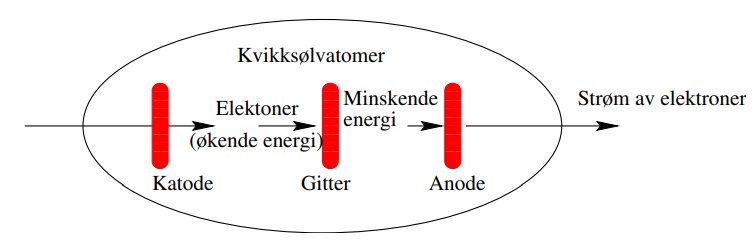
\includegraphics[scale = .7]{Figures/Franck-Hertz Eksperiment.png}
  \caption{Franck Hertz eksperimentet}
  \label{fig: Frank Hertz}
\end{figure}
Ved gitteret er det positivt potensialet som blir negativt mot katoden og anoden. Den totale spenning $V$ er gitt ved 
\[
V = V_{\text{KG}} - I V_{\text{GA}}I
\]
Elektronene Reiser fra Katoden og mister litt energi over gitteret. Mister de for mye energi vil de ikke kunne komme seg til anoden. Hvis spenningen øktes vil kollisjonen i gitteret ha mindre effekt og det øker sjansen for å komme seg til anoden. Dette varer frem til spesifikk spenninger hvor vi ser en dip i antall elektroner som når frem til anoden. Dette er fordi at elektronene får nok energi til å eksitere elektronene i atomene i gitteret, og mister dermed ekstremt mye mer energi enn vanlig. Noen elektroner vil likevel kunne både eksitere og komme seg til anoden. Ved å øke spenningen enda mer vil vi på nytt se en reduksjon av strøm ettersom elektronene eksiterer enda et elektron i et nytt atom i gitteret. De eksiterte elektronene vil falle ned til sin grunntilstand i et laver skall og vil sende ut ut energien i form av lys. 

\paragraph{Oppsumering}
\begin{itemize}
    \item Antar eksistensen av stasjonære tilstander
    \item Antar at elektronet i de sirkulære banene, og da er angulærmomentum kvantisert med $L = mvr = n ℏ$
    \item Lyktes spektakulært med å forutsi atomspekteret og de kjemiske egenskapene til enkle atomer 
    \item Idéen om elektronbaner blir modifisert av kvantemekanikken
\end{itemize}
